\documentclass{amsart}
\usepackage{latexsym,amscd,amssymb, graphicx, amsthm,amsmath}
\usepackage{tikz-cd, xcolor}
\usetikzlibrary{calc}
\usetikzlibrary{decorations.markings}

\begin{document}

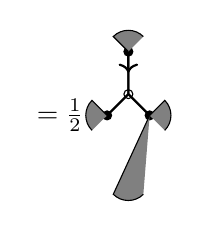
\begin{tikzpicture}[scale = .27]
  % Left-hand side label
  \node at (-3.2,-3) {$=\frac{1}{2}$};

  % Draw main node circles (define key points first for clarity)
  \draw[fill = black] (0,0) circle (6pt);        % Top vertex
  \draw[fill = white] (0,-2) circle (6pt);       % Middle vertex
  \draw[fill = black] (-1,-3) circle (6pt);      % Bottom-left vertex
  \draw[fill = black] (1,-3) circle (6pt);       % Bottom-right vertex

  % Draw connecting edges
  \draw[thick,->] (0,0)--(0,-1);                 % Arrow from top to middle
  \draw[thick] (0,0)--(0,-2)--(-1,-3);           % Left branch
  \draw[thick] (0,0)--(0,-2)--(1,-3);            % Right branch

  % Draw gray arcs around vertices
  \draw[fill = gray] (-1,-3)--(-1.71,-2.29) arc (135:225:1);   % Arc at bottom-left
  \draw[fill = gray] (1,-3)--(1.71,-2.29) arc (45:-45:1);      % Arc at bottom-right
  \draw[fill = gray] (0,0)--(-.71,.71) arc (135:45:1);         % Arc at top
  \draw[fill = gray] (1,-3)--(-.71,-6.71) arc (225:315:1);     % Arc below bottom-right
\end{tikzpicture}

\end{document}